\documentclass{article}


 % Required for inserting code snippets
\usepackage{mathtools}
\usepackage{graphicx}
\usepackage{subfig}
\usepackage{verbatim}
\usepackage{algpseudocode}
\usepackage{natbib}
\usepackage{url}
\usepackage{listings}
\usepackage{float}
\usepackage{array}
\usepackage{booktabs}
\usepackage{amssymb}
%\setcounter{MaxMatrixCols}{16}

%%%%%%%%%%%%%%%%%%%%%%%% PAINTING LIBRARY
\usepackage{pgf}
\usepackage{tikz}
\usetikzlibrary{arrows,automata}
\usepackage[latin1]{inputenc}
\usepackage[upright]{fourier}
\usetikzlibrary{matrix}
\usepackage{fullpage,amsmath}

%%%%%%%%%%%%%%%%%%%%%%%% THNX TO OZAN FOR THE CODE HEADER ;)
\usepackage{color}
\usepackage{xcolor}
\usepackage{listings}

\usepackage{courier}
\definecolor{DarkGray}{rgb}{0.43,0.35,0.35} % Comment color
\lstset{
	language=C++,								% choose the language of the code
		basicstyle=\footnotesize\ttfamily,  % the size of the fonts that are used for the code
		numbers= left,						% where to put the line-numbers
		numberstyle=\tiny,					% the size of the fonts that are used for the line-numbers
		stepnumber=1,						% the step between two line-numbers. If it is 1 each line will be numbered
		numbersep=10pt,						% how far the line-numbers are from the code
		backgroundcolor=\color{white},		% choose the background color. You must add \usepackage{color}
		keywordstyle=\color{DarkGray}\bf,
	showspaces=false,						% show spaces adding particular underscores
		showstringspaces=false,				% underline spaces within strings
		showtabs=false,						% show tabs within strings adding particular underscores
		keywordstyle=\color{DarkGray}\bf,
		stringstyle=\color[rgb]{0.627,0.126,0.941},
		xleftmargin=17pt,
		framexleftmargin=17pt,
		framexrightmargin=5pt,
		framexbottommargin=4pt,
		%frame=b,         
		frame=single,					% adds a frame around the code
		tabsize=2,						% sets default tabsize to 2 spaces
		captionpos=t,					% sets the caption-position to bottom (t=top, b=bottom)
		breaklines=true,				% sets automatic line breaking
		breakatwhitespace=false,		% sets if automatic breaks should only happen at whitespace
		escapeinside={\%*}{*)}          % if you want to add a comment within your code
}

\usepackage{caption}
\DeclareCaptionFont{white}{\color{white}}
\DeclareCaptionFormat{listing}
{
	\colorbox[rgb]{0.83, 0.85, 0.88}
	{\parbox{\dimexpr\textwidth-8\fboxsep\relax}{#1#2#3}}
}

\captionsetup[lstlisting]
{
	format=listing,
		labelfont=white,
		textfont=white, 
		singlelinecheck=false, 
		margin=0pt, 
		font={bf,footnotesize}
}

\usepackage{textcomp}

%%%%%%%%%%%%% WATERMARKS  %%%%%%%%%%%%%%%%%
%\usepackage{eso-pic}
%\AddToShipoutPicture{
%    \includegraphics[width=1.74\textwidth,natwidth=1223,natheight=121]{figs/lowImg2.png}}

\DeclarePairedDelimiter\abs{\lvert}{\rvert}


%%%%%%%%%%%%% PARAGRAPHS %%%%%%%%%%%%%%%%%
%No ident in new paragraph
\usepackage[parfill]{parskip}
%% Add a space of 1.5 lines between paragraphs
\parskip=1.1\baselineskip

%%%%%%%%%%%%% DEFAULT FONT %%%%%%%%%%%%%%%
%Sans-serif font by default
%\renewcommand{\familydefault}{\sfdefault}
%\usepackage{mathptmx}

%\usepackage{bookman}
%%%%%\usepackage[default]{droidserif}
%\usepackage[T1]{fontenc}
%\usepackage{lxfonts}
%\usepackage{tgadventor}
%\renewcommand*\familydefault{\sfdefault} %% Only if the base font of the document is to be sans serif
%\usepackage[T1]{fontenc}


\newcommand{\specialcell}[2][c]{%
  \begin{tabular}[#1]{@{}c@{}}#2\end{tabular}}

\usepackage{float}



\begin{document}
\title{Polarization Imaging Report (Lab 1)}
\date {\today}
\author{Tatiana Lopez Guevara\\Klemen Istenic}
%\author{Tatiana Lopez Guevara}
\maketitle

\section{Simplified Polarization Imaging}

We used the configuration as illustrated on the picture 1 of the 
instructions:

%\begin{figure}[h!]
\begin{wrapfigure}{r}{0.3\textwidth}
\caption{}
\centering
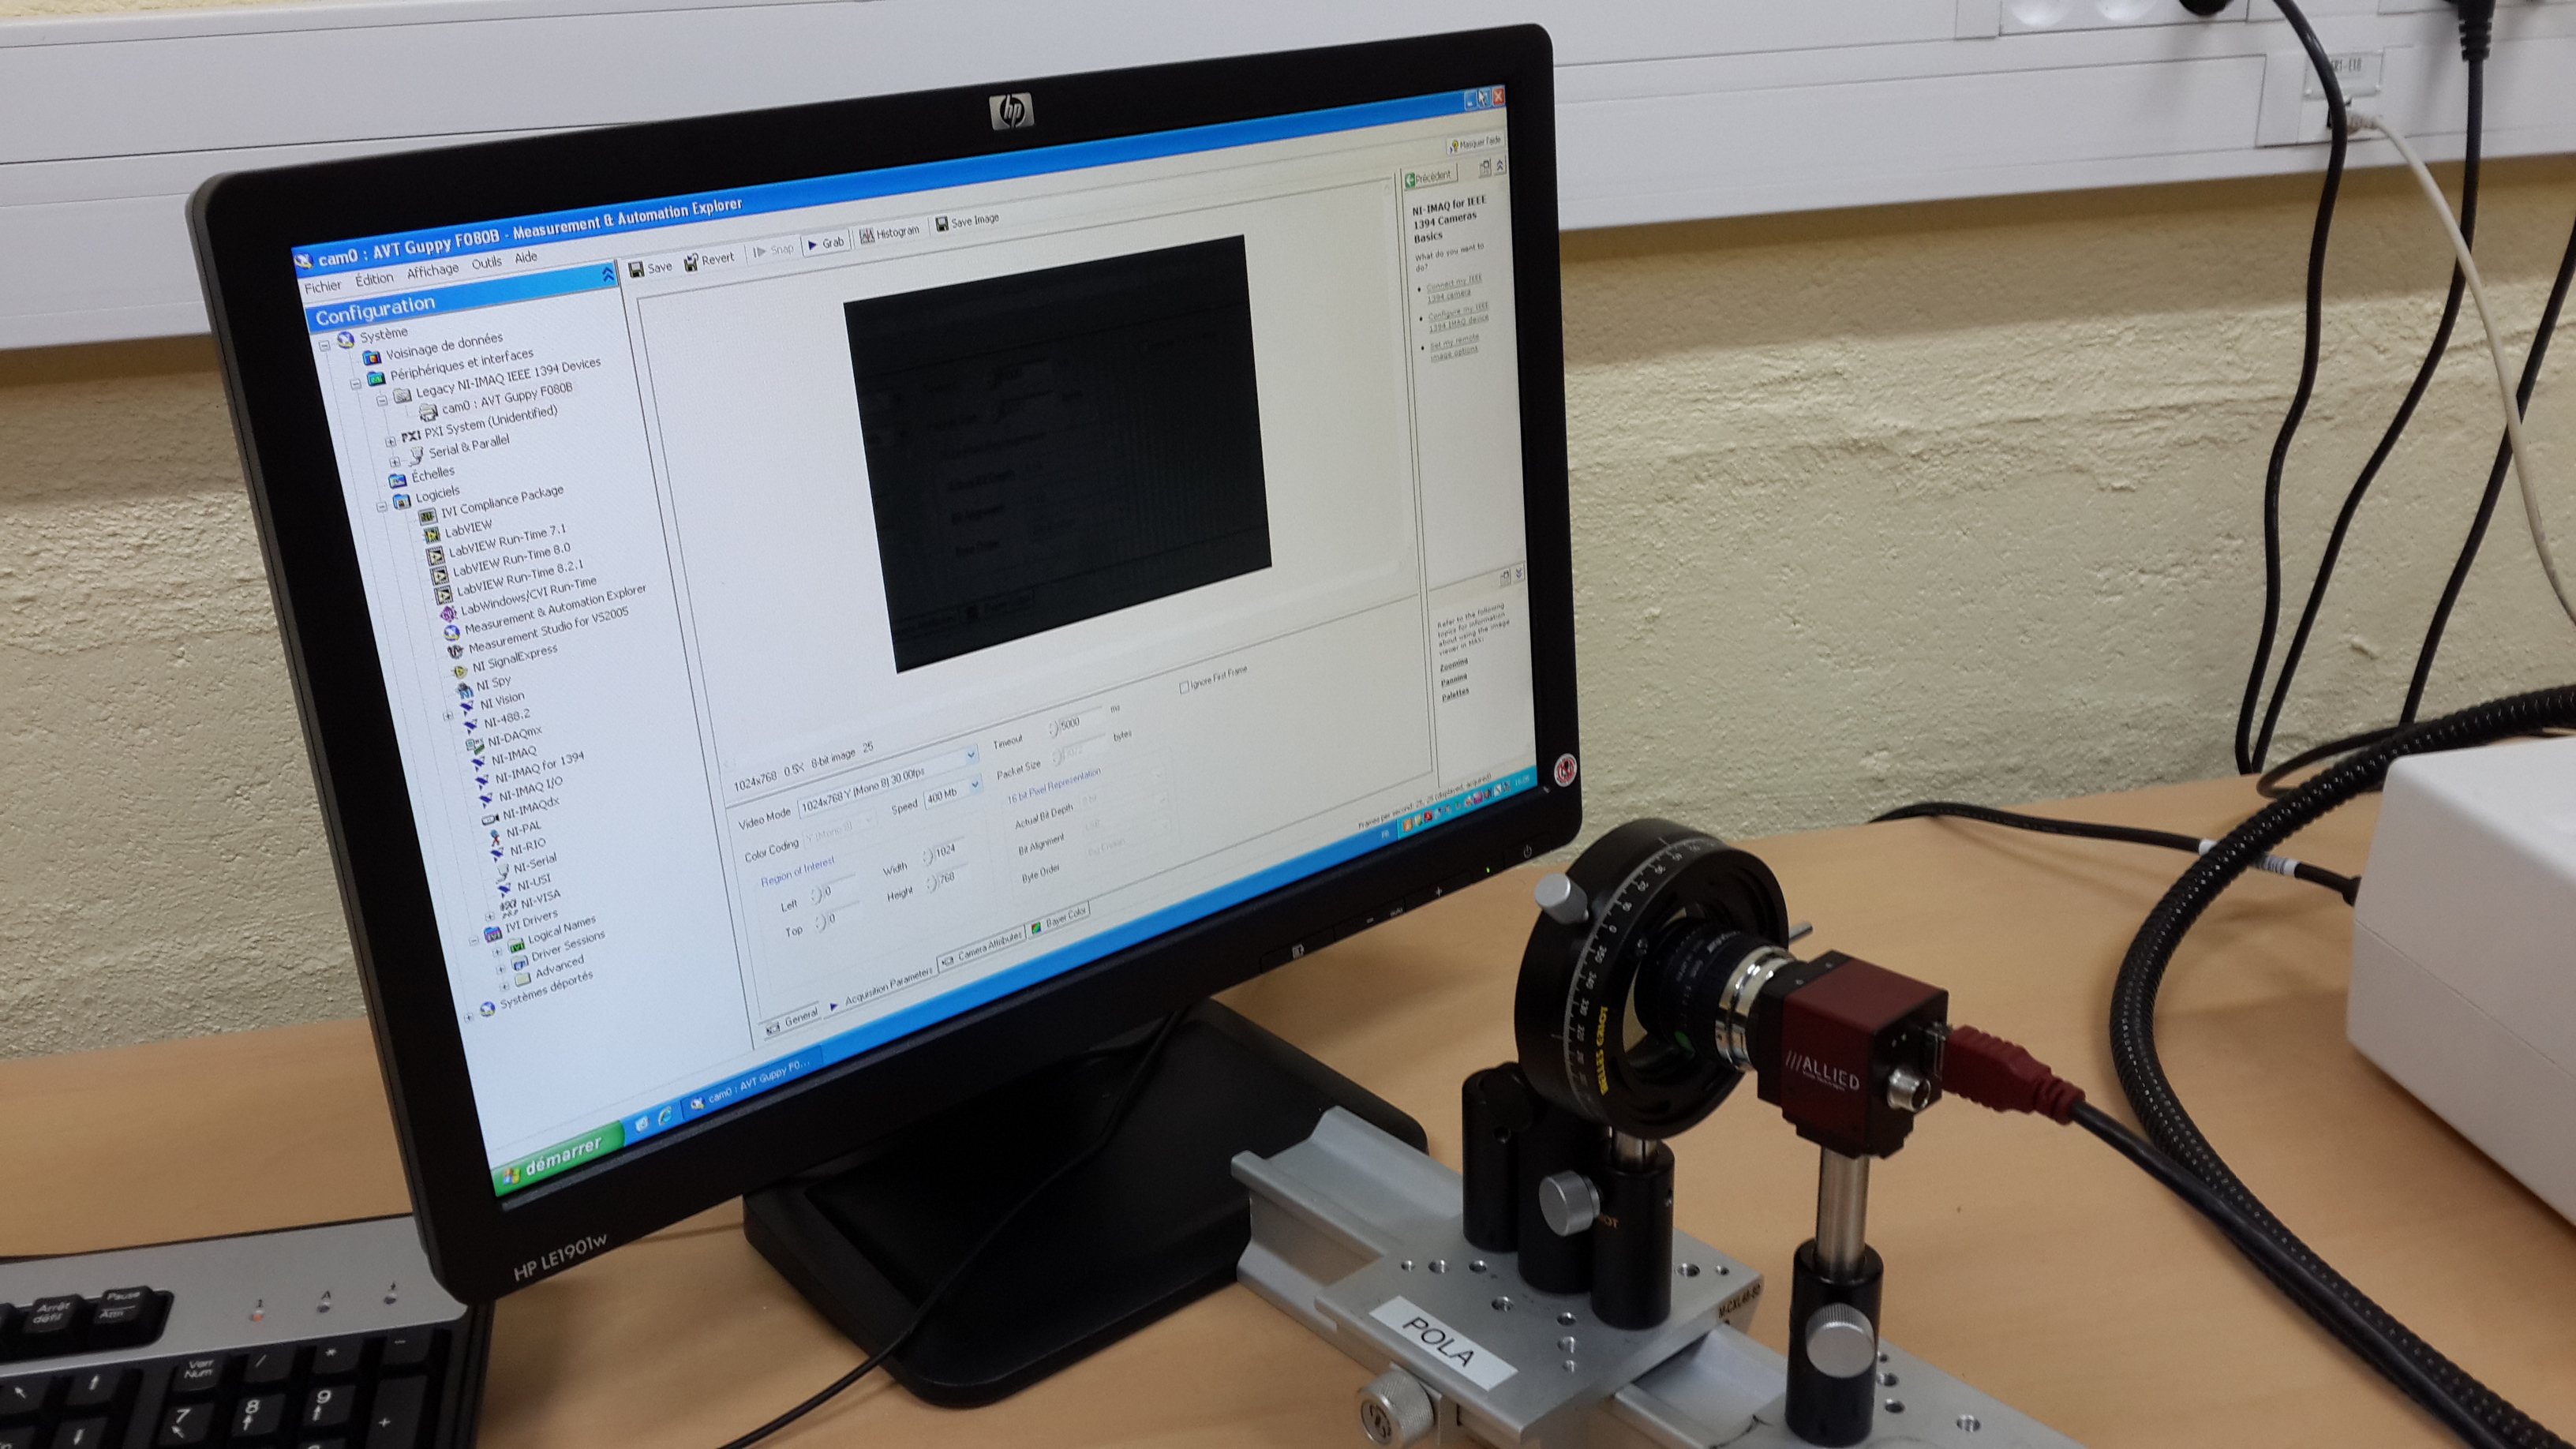
\includegraphics[width=0.48\textwidth,natwidth=100,natheight=100]{../photos/s1.jpg}
\label{fig:}
%\end{figure} 
\end{wrapfigure}

Because we wanted to see the difference the rotation of the polarizer has 
on polarized light and unpolarized light, we set up our camera so the computer
screen was captured only on one part of the image. 
We did this because we knew that the light coming from the computer
screen is linearly polarized. Moreover, we suspected the orientation polarization
is at 45$^\circ$ (as it is on most of the computer screens).

Initially our polarized was oriented at 0$^\circ$. As we were rotating it clockwise,
 the intesity on the part of the image showing the screen was increasing until 
it reached the maximum at 45$^\circ$. After that, the intensity started to decrease
until it was totally blocked at 135$^\circ$. We also noticed that the intesity
at 90$^\circ$ was the same as the intensity at 0$^\circ$.

This shows that the light coming from the screen was in fact polarized
at 45$^\circ$ because when both, angle of polarized light and the polarizer
are aligned, a maximum is achieved as none of the light is blocked by the polarizer.
In contrast, at 135$^\circ$ the angle between them was orthogonal so everything
was blocked and the intesity on the resulting image is 0.

\subsection{Wollf's Method}

In the camera settings, autoexposure means that the exposure is 
automatically adjusted according to the ambient light of the scene.
Auto Gain Control (AGC) increases the intensifier gain if the video 
scene is too dim and decreases the gain if the scene is too bright
\cite{fowler2004automatic}.

We can see in the following 2 figures that when autoexposure and AGC are enabled,
the camera automatically tries to compensate for brightnes.
Since we needed to maintain the consistency between the measurements,
these parameters were turned off.

\begin{figure}[ht]
\centering
\begin{minipage}[b]{0.3\linewidth}
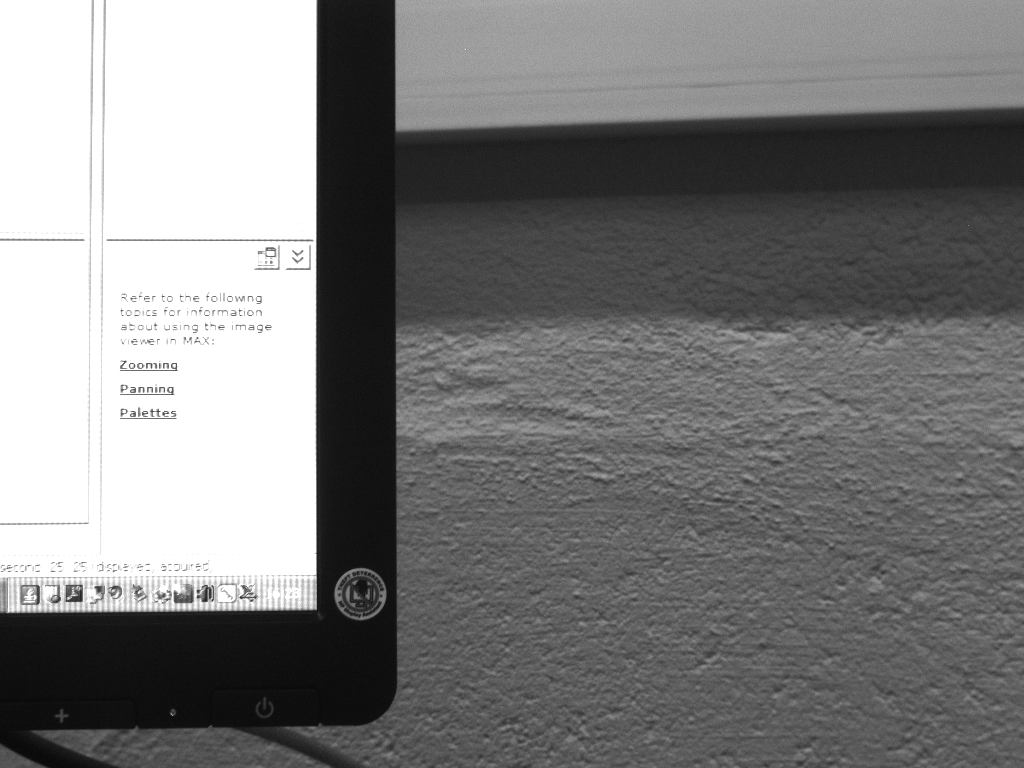
\includegraphics[width=1.0\textwidth,natwidth=100,natheight=100]{gainAuto.png}
  \caption{AutoGain On}
  \label{fig:minipage1}
\end{minipage}
\quad
\begin{minipage}[b]{0.3\linewidth}
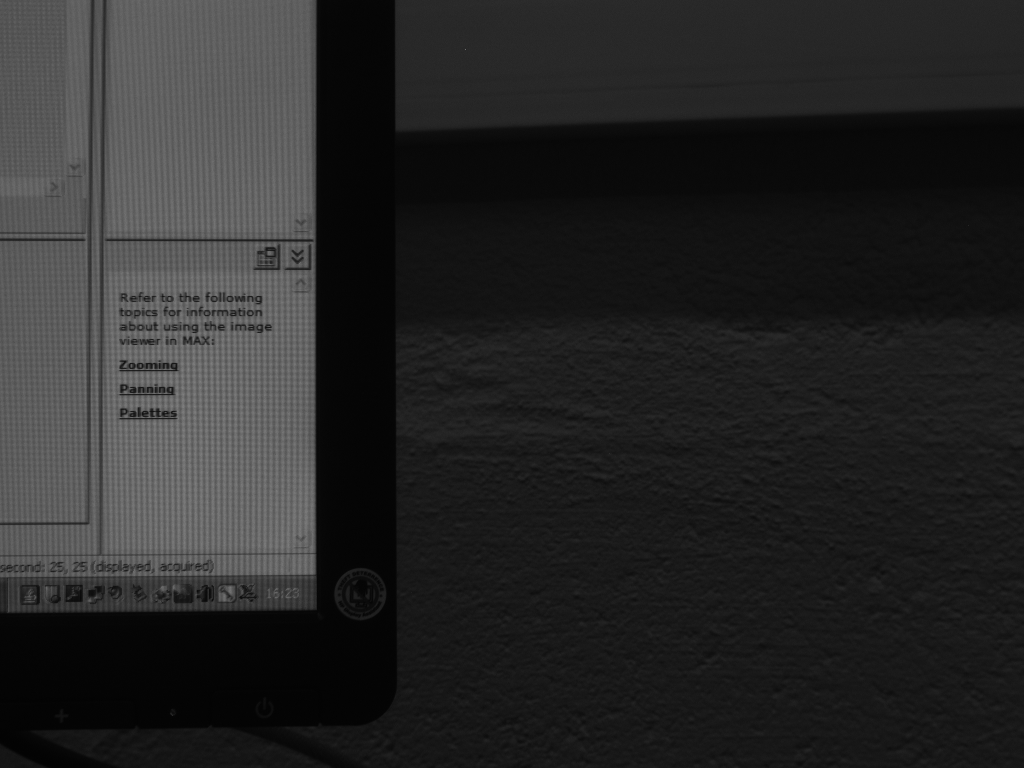
\includegraphics[width=1.0\textwidth,natwidth=100,natheight=100]{gainManual.png}
  \caption{AutoGain Off}
  \label{fig:minipage2}
\end{minipage}
\end{figure}

Figures \ref{fig:wolf1-1}, \ref{fig:wolf1-2} and \ref{fig:wolf1-3} show our images
taken at 0$^\circ$, 45$^\circ$ and 90$^\circ$ respectively. After the capture, 
we noticed some stripes due to the position of the camera and because of the lower 
resolution of display in the program we didnt noticed it during 
the labs.  Therefore, the obtained parameters
for the intensity, angle of polarization $\phi$ 
and degree of polarization $\rho$ were calculated only on the non
corrupted pixels for each region of interest
 shown in figure \ref{fig:wolf1-4} 
obtaining the results given by the table \ref{tb:wolffres}.

\begin{figure}[H]
\centering
\begin{minipage}[b]{0.18\linewidth}
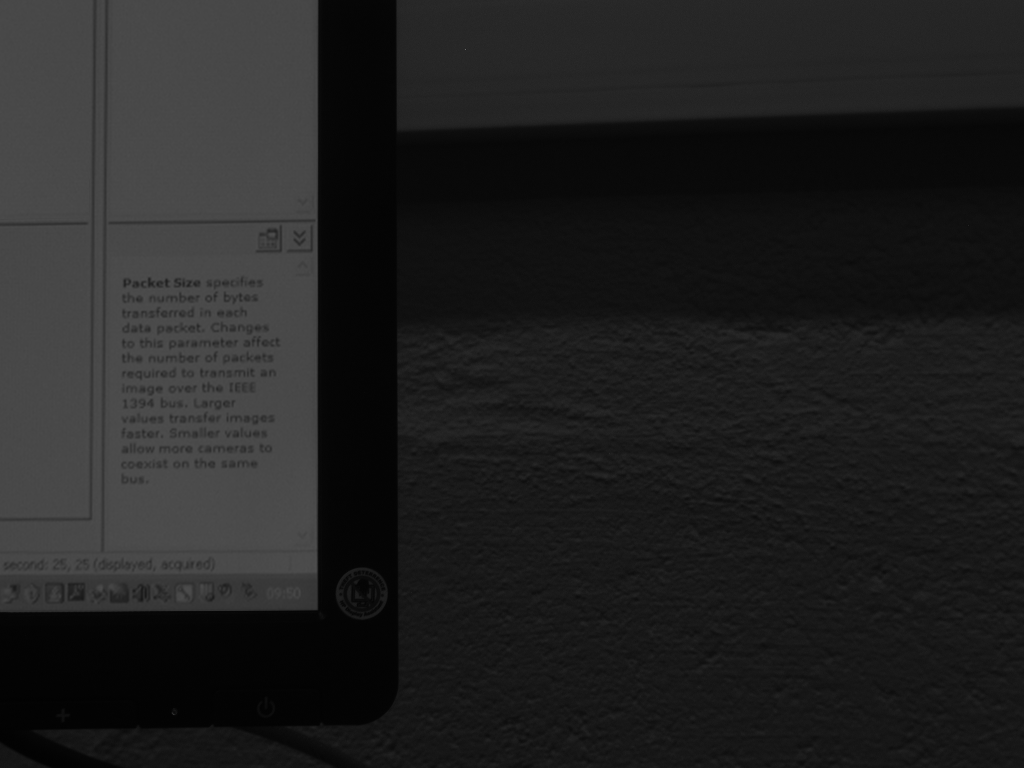
\includegraphics[width=1.0\textwidth,natwidth=100,natheight=100]{../wolff/results/im0.png}
  \caption{Polarizer at 0$^\circ$}
  \label{fig:wolf1-1}
\end{minipage}
\quad
\begin{minipage}[b]{0.18\linewidth}
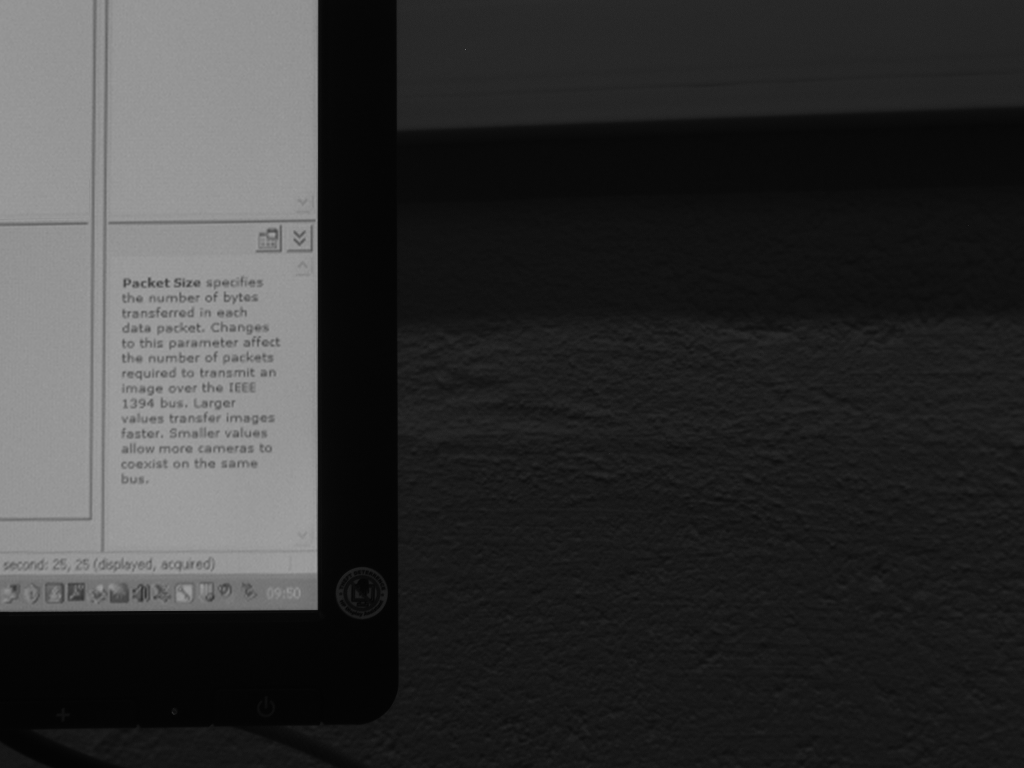
\includegraphics[width=1.0\textwidth,natwidth=100,natheight=100]{../wolff/results/im45.png}
  \caption{Polarizer at 45$^\circ$}
  \label{fig:wolf1-2}
\end{minipage}
\quad
\begin{minipage}[b]{0.18\linewidth}
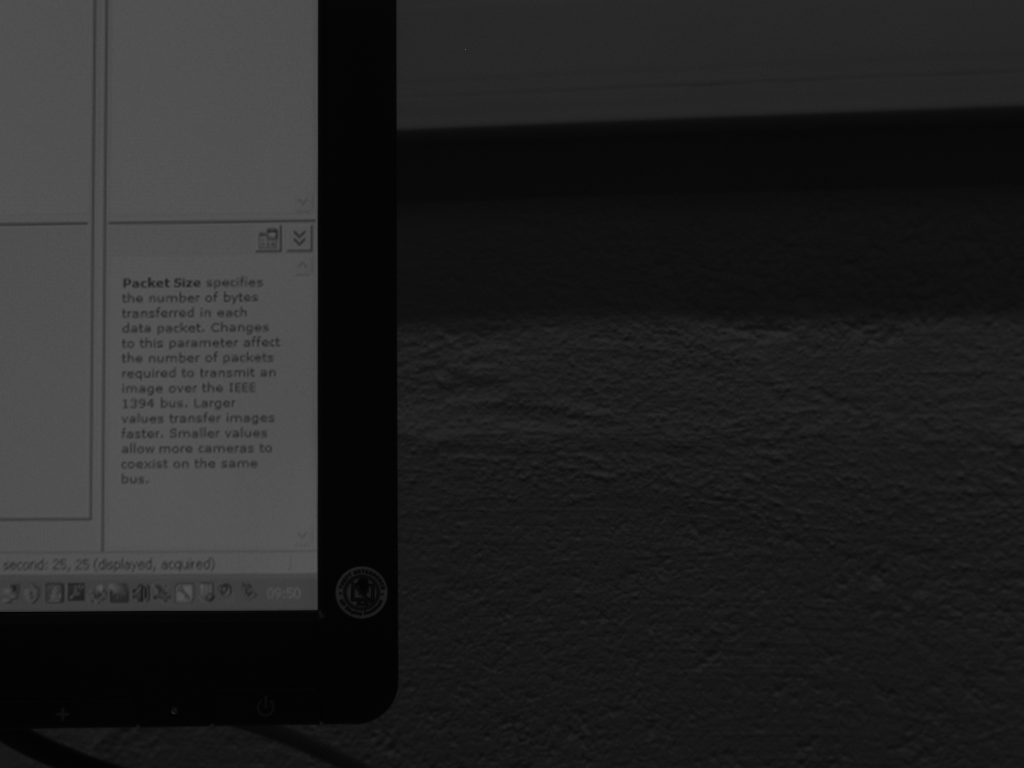
\includegraphics[width=1.0\textwidth,natwidth=100,natheight=100]{../wolff/results/im90.png}
  \caption{Polarizer at 90$^\circ$}
  \label{fig:wolf1-3}
\end{minipage}
\quad
\begin{minipage}[b]{0.18\linewidth}
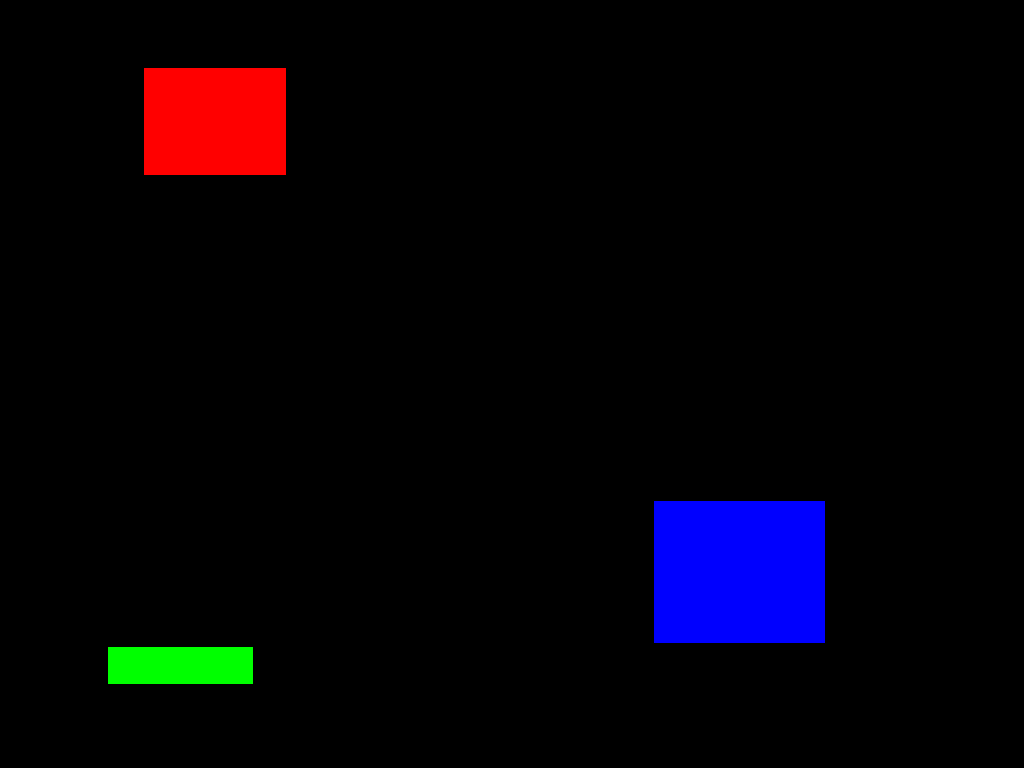
\includegraphics[width=1.0\textwidth,natwidth=100,natheight=100]{../wolff/results/mask.png}
  \caption{Regions of Interest (Mask)}
  \label{fig:wolf1-4}
\end{minipage}
\end{figure}

\begin{table}
\centering
\begin{tabular}{|c|c|c|c|c|}
\hline
Region & Mask Color & I & $\phi$ & $\rho$ \\ 
\hline
Border & Green & 6.744471 & -0.529405 &  0.441451 \\
Background & Blue & -0.060872 & -3.48 & 0.060838\\
Screen (filtered) & Red & 153.000000 & -0.781801 & 0.908520\\
\hline
\end{tabular}
\caption{Obtained results for different Regions of Interest (ROI)}
\label{tb:wolffres}
\end{table} 

In order to display the polarization parameteres we used the HSL representation
by performing the following mapping: $H \to 2\phi$, $S \to I$ and $L\to\rho$ as 
in the slides.
The result is shown in figure \ref{fig:hsl}.

\begin{figure}[H]
\caption{HSL representation of Polarization}
\centering
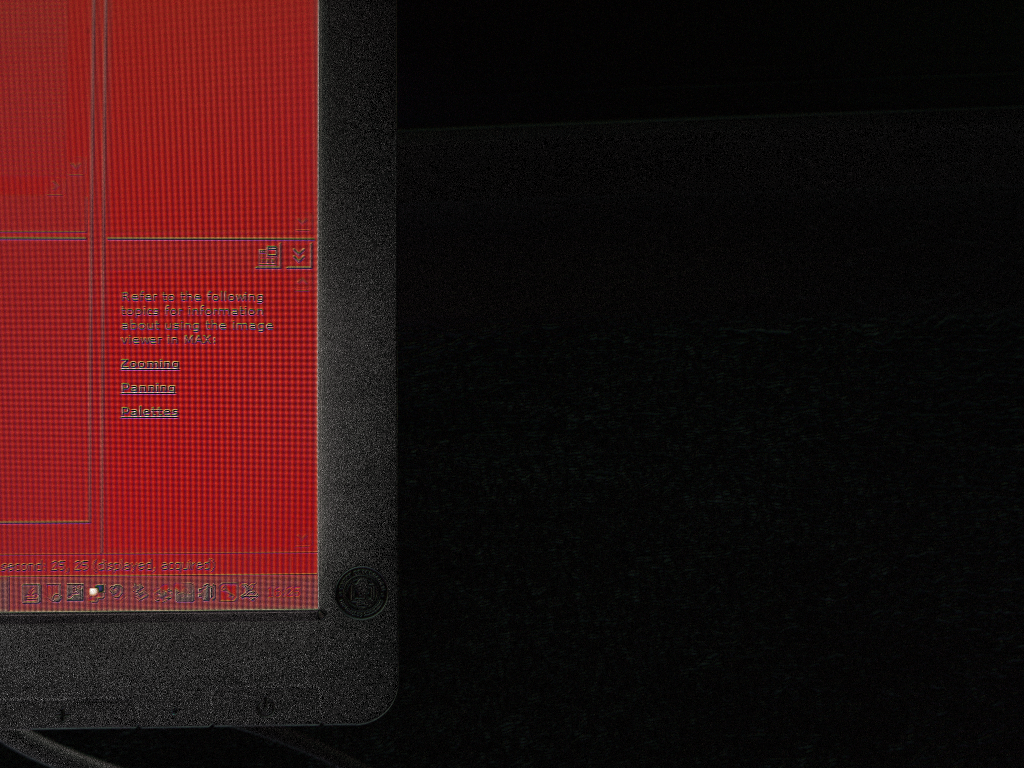
\includegraphics[width=0.4\textwidth,natwidth=100,natheight=100]{../wolff/results/result_wolff.png}
\label{fig:hsl}
\end{figure}   

\subsection{Least Mean Square Method}

In this section we took 10 different measurements with different rotations of the 
polarizer as shown in the figures \ref{fig:lms11-1} to \ref{fig:lms11-10} in order to get 
a better approximation of the polarization parameters.

\begin{figure}[H]
\centering
\begin{minipage}[b]{0.16\linewidth}
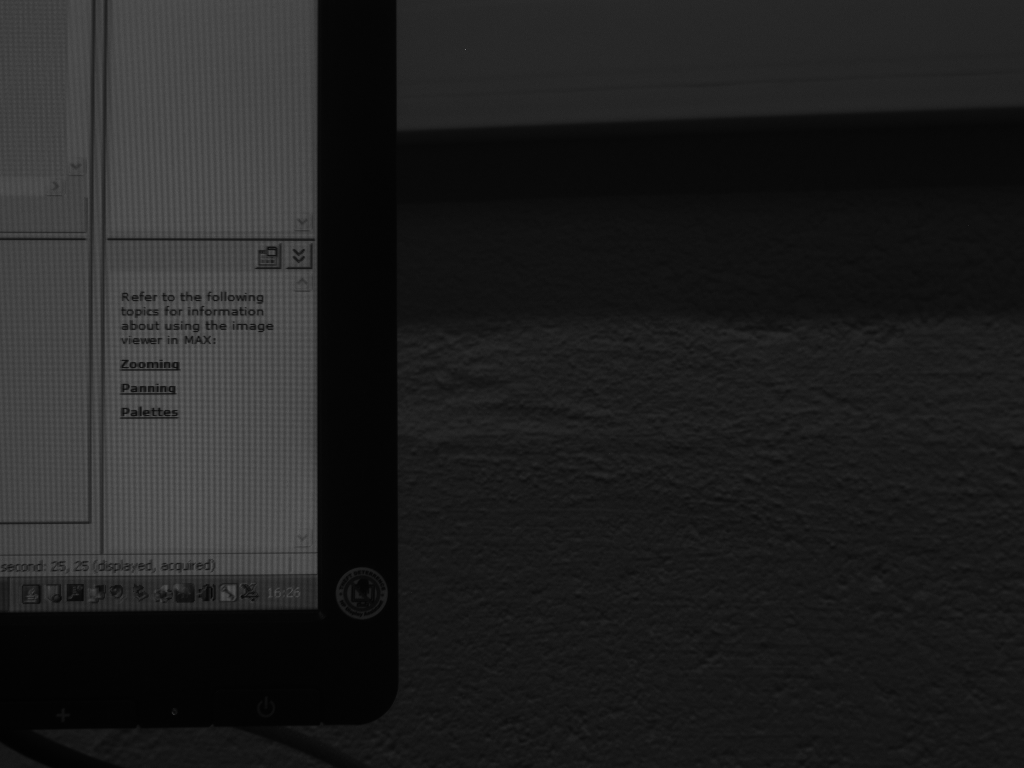
\includegraphics[width=1.0\textwidth,natwidth=100,natheight=100]{../LMS/im0.png}
  \caption{0$^\circ$}
  \label{fig:lms11-1}
\end{minipage}
\quad
\begin{minipage}[b]{0.16\linewidth}
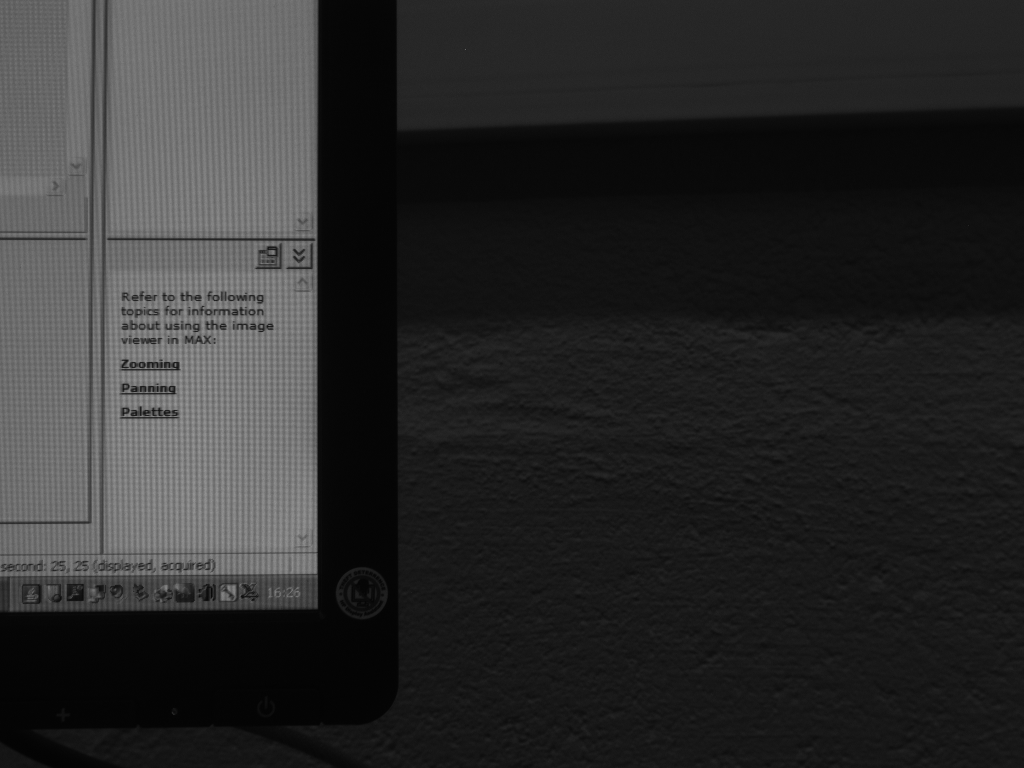
\includegraphics[width=1.0\textwidth,natwidth=100,natheight=100]{../LMS/im20.png}
  \caption{20$^\circ$}
  \label{fig:lms11-2}
\end{minipage}
\quad
\begin{minipage}[b]{0.16\linewidth}
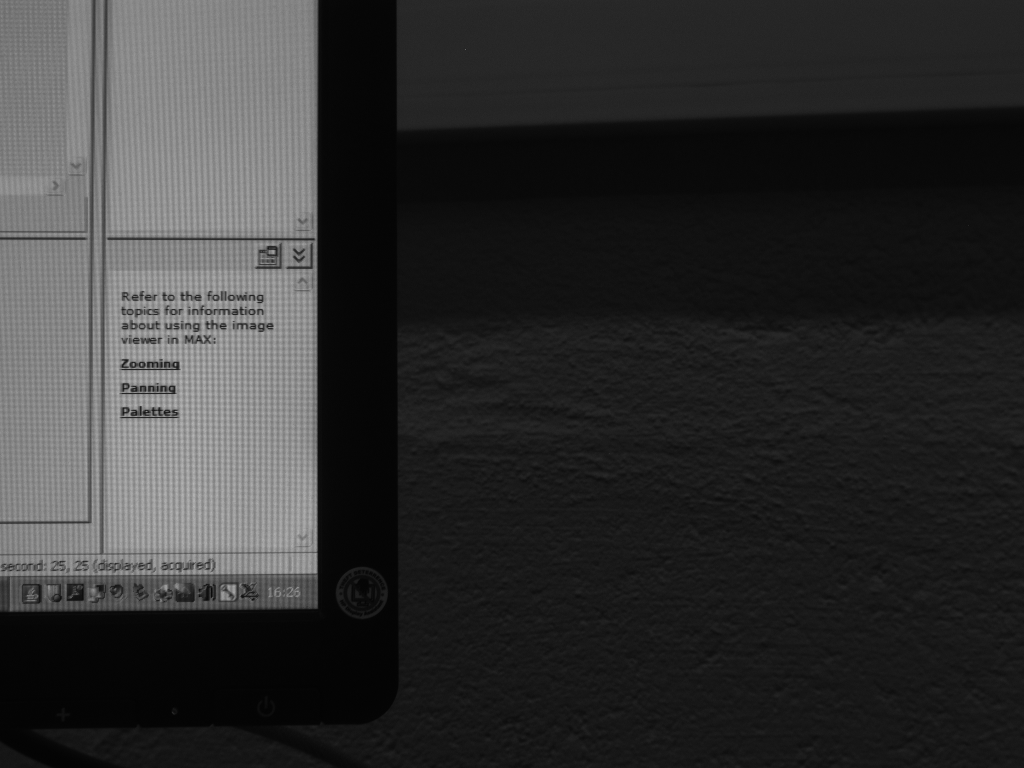
\includegraphics[width=1.0\textwidth,natwidth=100,natheight=100]{../LMS/im40.png}
  \caption{40$^\circ$}
  \label{fig:lms11-3}
\end{minipage}
\quad
\begin{minipage}[b]{0.16\linewidth}
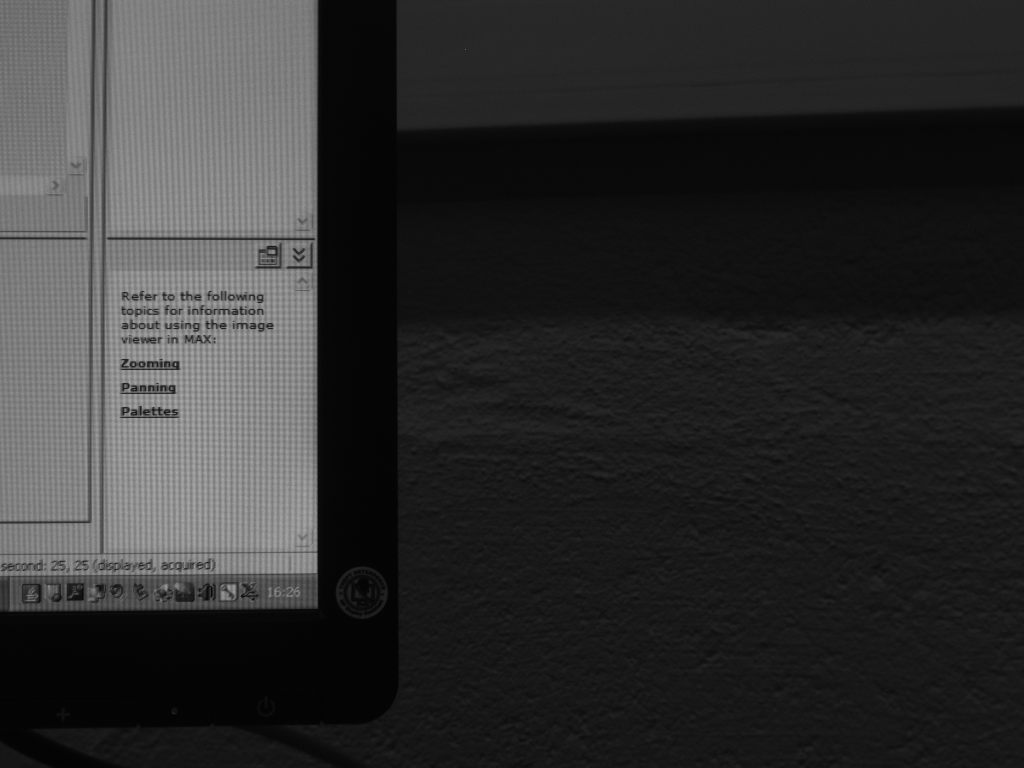
\includegraphics[width=1.0\textwidth,natwidth=100,natheight=100]{../LMS/im60.png}
  \caption{60$^\circ$}
  \label{fig:lms11-4}
\end{minipage}
\quad
\begin{minipage}[b]{0.16\linewidth}
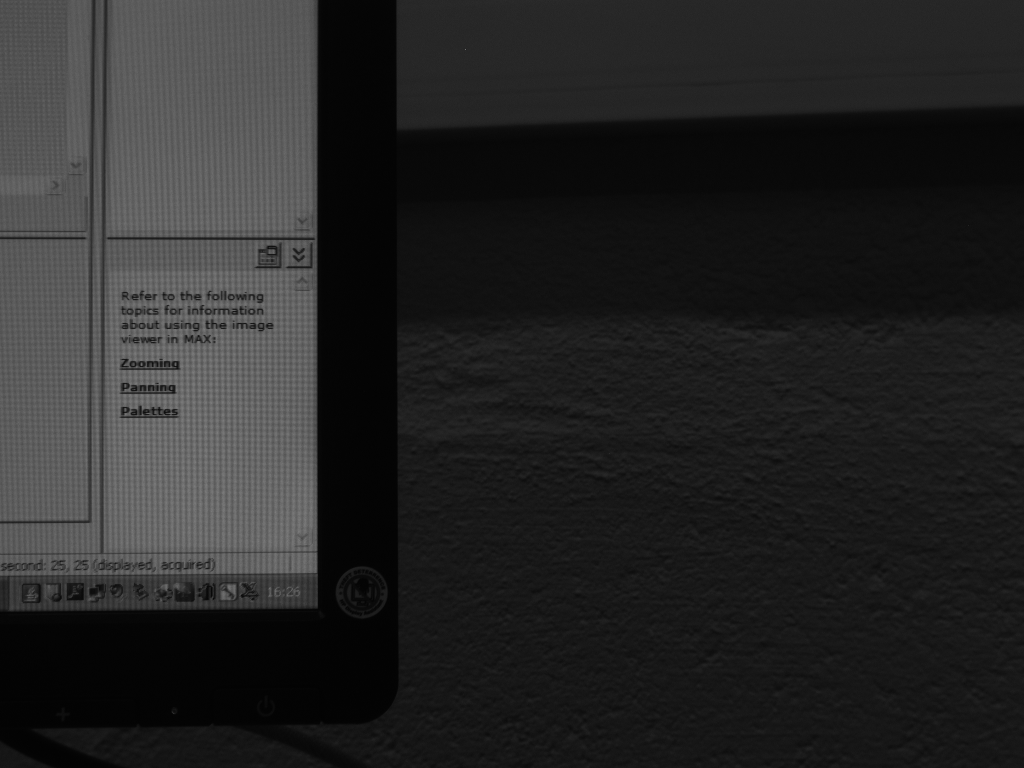
\includegraphics[width=1.0\textwidth,natwidth=100,natheight=100]{../LMS/im80.png}
  \caption{80$^\circ$}
  \label{fig:lms11-5}
\end{minipage}
\quad
\begin{minipage}[b]{0.16\linewidth}
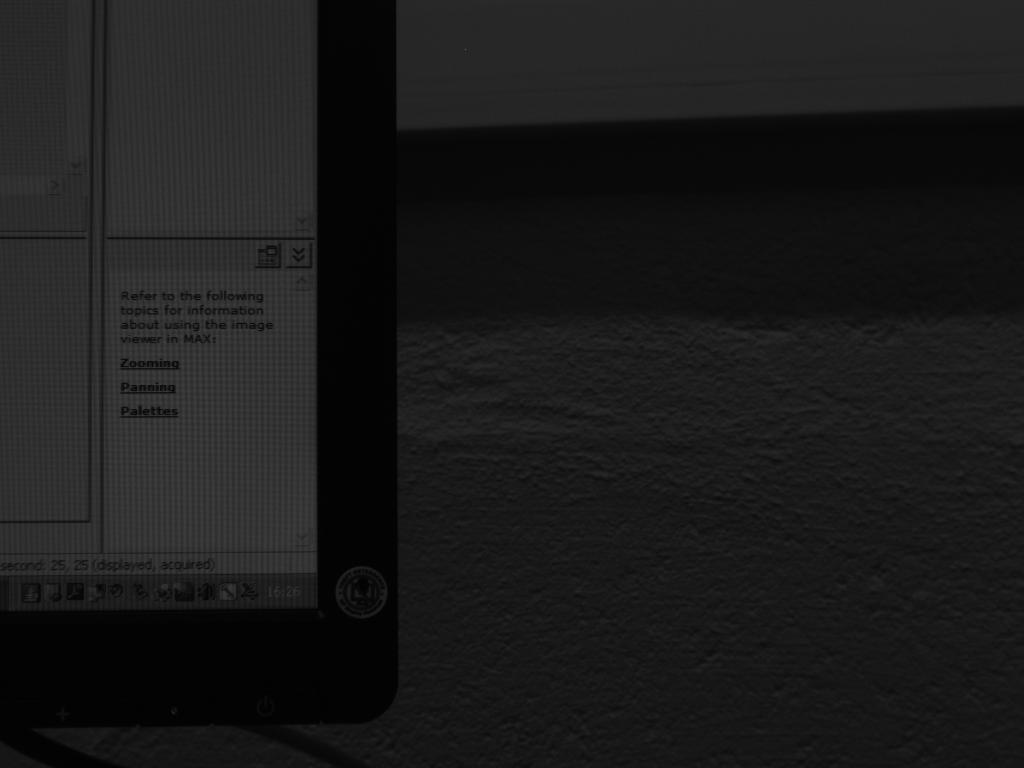
\includegraphics[width=1.0\textwidth,natwidth=100,natheight=100]{../LMS/im100.png}
  \caption{100$^\circ$}
  \label{fig:lms11-6}
\end{minipage}
\quad
\begin{minipage}[b]{0.16\linewidth}
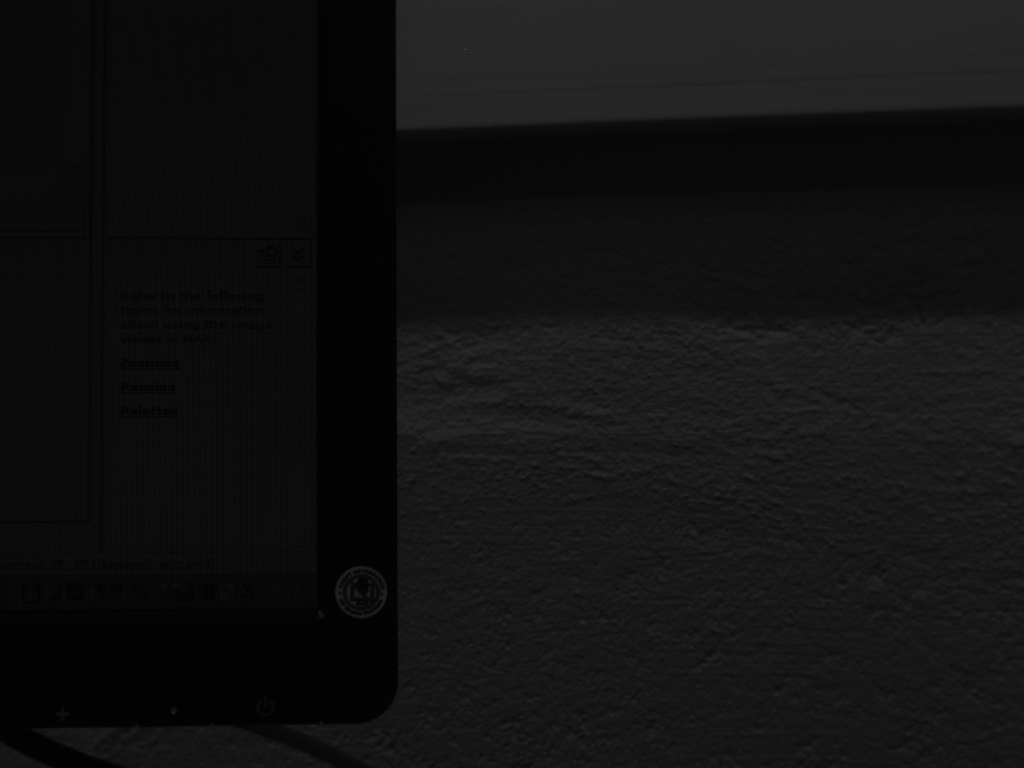
\includegraphics[width=1.0\textwidth,natwidth=100,natheight=100]{../LMS/im120.png}
  \caption{120$^\circ$}
  \label{fig:lms11-7}
\end{minipage}
\quad
\begin{minipage}[b]{0.16\linewidth}
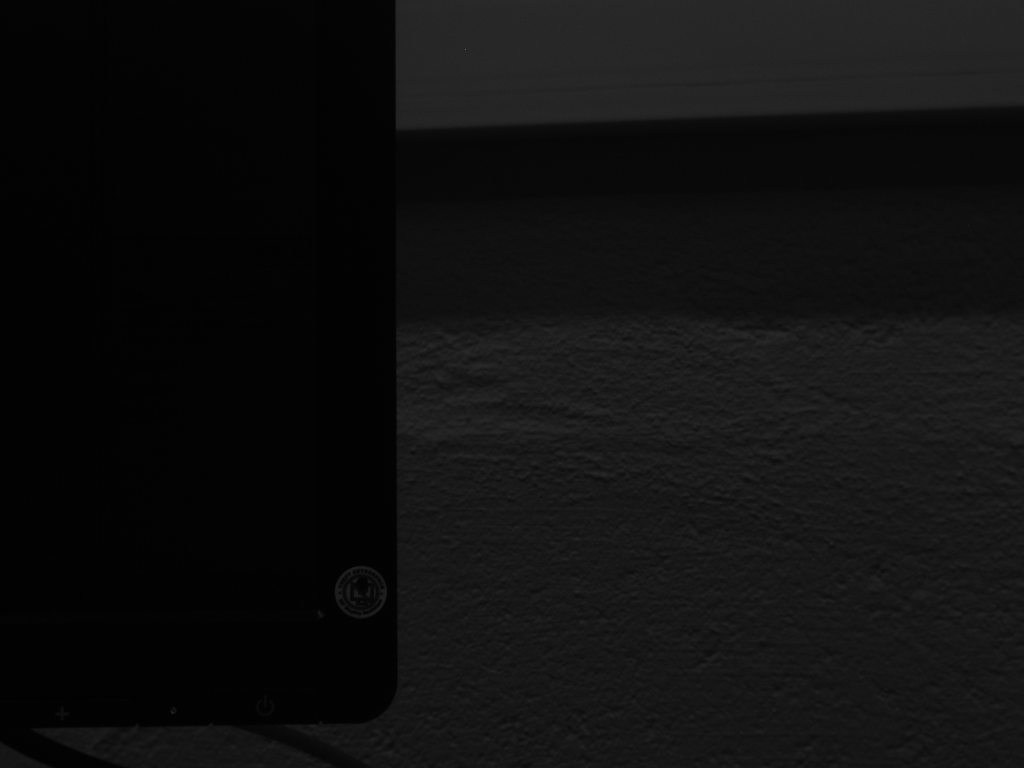
\includegraphics[width=1.0\textwidth,natwidth=100,natheight=100]{../LMS/im140.png}
  \caption{140$^\circ$}
  \label{fig:lms11-8}
\end{minipage}
\quad
\begin{minipage}[b]{0.16\linewidth}
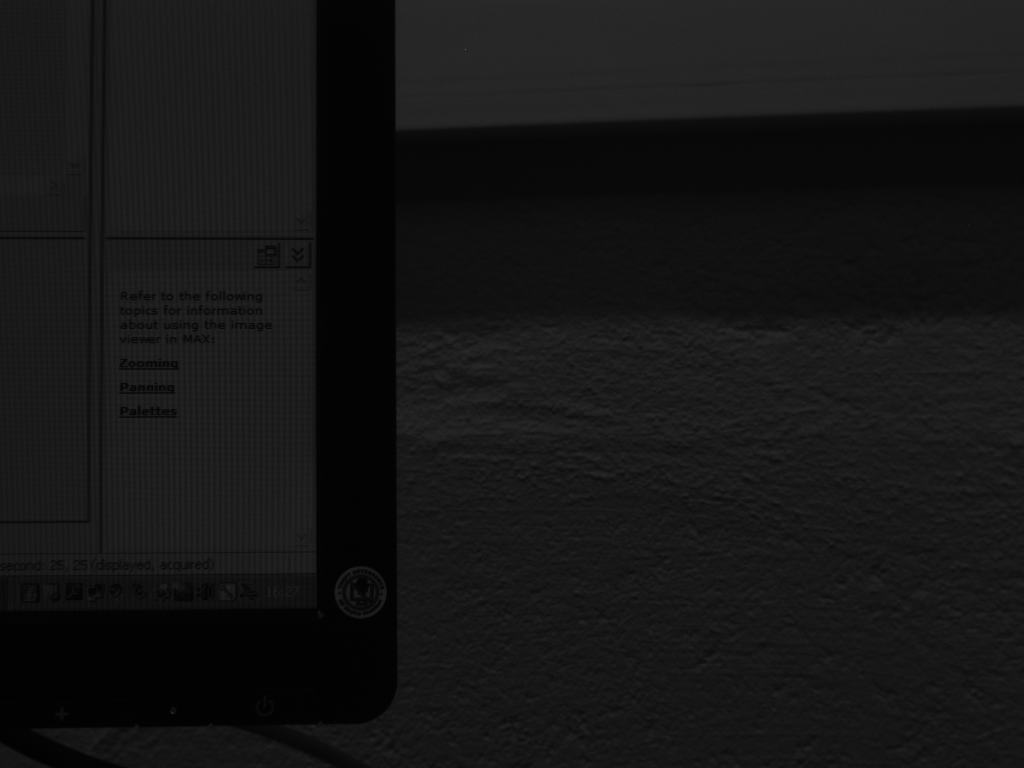
\includegraphics[width=1.0\textwidth,natwidth=100,natheight=100]{../LMS/im160.png}
  \caption{160$^\circ$}
  \label{fig:lms11-9}
\end{minipage}
\quad
\begin{minipage}[b]{0.16\linewidth}
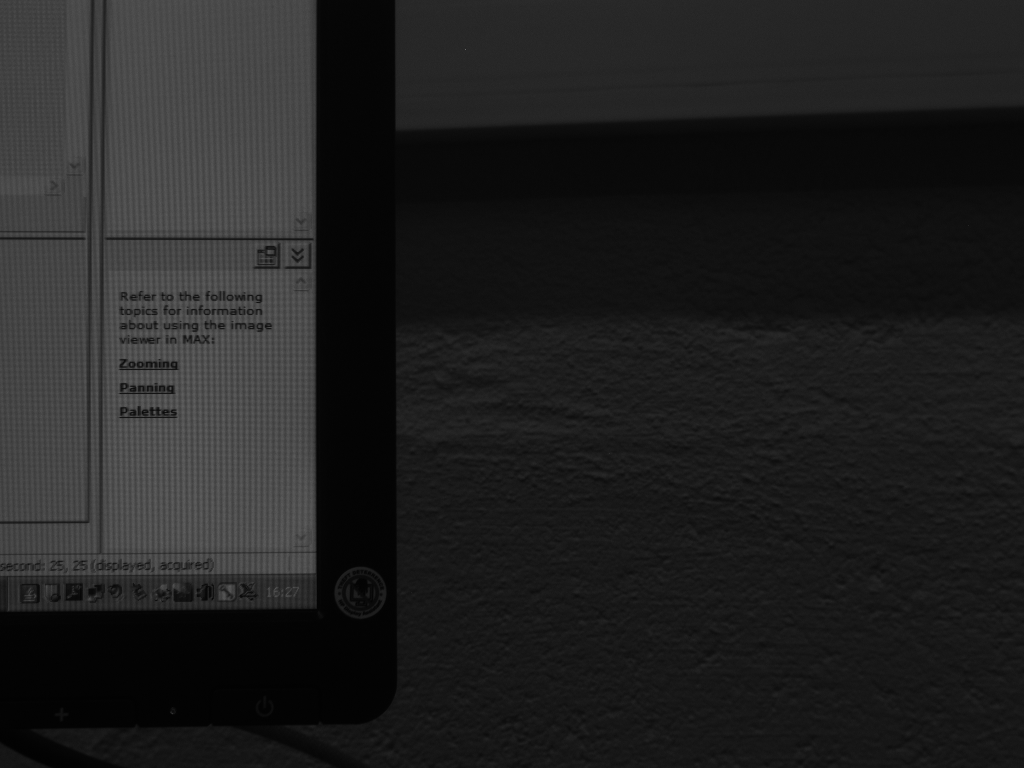
\includegraphics[width=1.0\textwidth,natwidth=100,natheight=100]{../LMS/im180.png}
  \caption{180$^\circ$}
  \label{fig:lms11-10}
\end{minipage}
\end{figure}

The obtained image after calculating the LMS with the 10 images is shown in the figure 
\ref{fig:hslms}.
For the analyzed pixels in the screen we obtained a sinusoidal relation as
can be seen in the figure \ref{fig:sin}.
This results are consecuent with the Malus Law $I=I_0 cos^2\alpha$ in which the
maximum intesity is obtained when the angle $\alpha$ of the polarizer matches 
the polarized light (at around 45$^\circ$) and none intensity where they are orthogonal
(around 135$^\circ$)..


\begin{figure}[H]
\centering
\begin{minipage}[b]{0.45\linewidth}
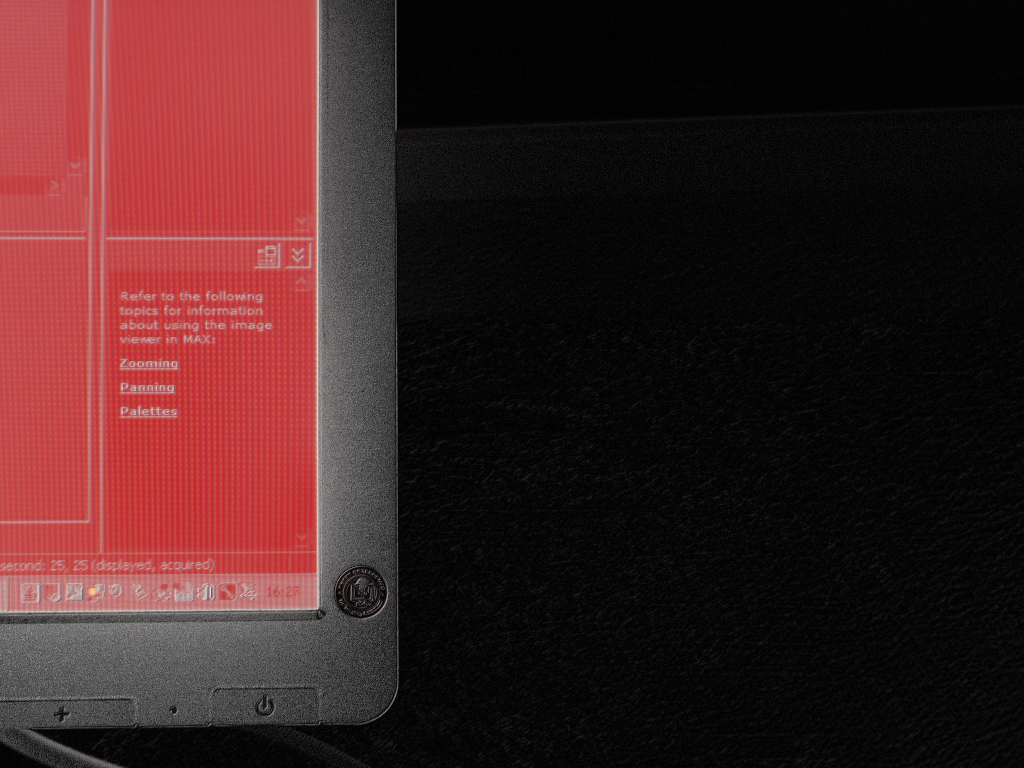
\includegraphics[width=1.0\textwidth,natwidth=100,natheight=100]{../LMS/results/result_lms.png}
\caption{HSL representation of LMS results}
\label{fig:hslms}
\end{minipage}
\quad
\begin{minipage}[b]{0.45\linewidth}
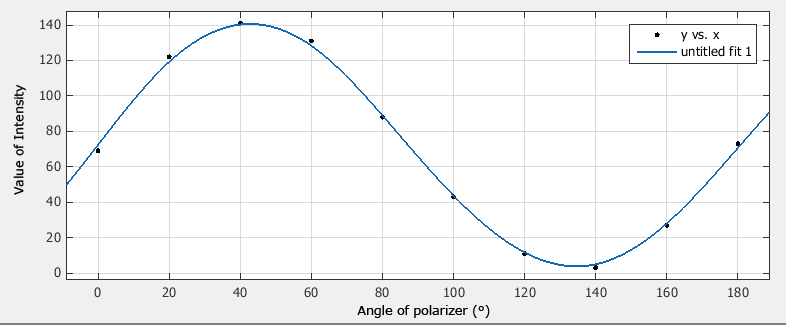
\includegraphics[width=1.2\textwidth,natwidth=100,natheight=100]{../LMS/results/sinus_wave.png}
\caption{Sinusoidal Wave of Single Pixel}
\label{fig:sin}
\end{minipage}
\end{figure}   
\section{Contrast Polarization Measurement}

The first thing we noticed was the difference of the obtained intensity of the image
when we used only one polarizer at 0$^\circ$ (figure \ref{fig:cpm1-1}) 
versus the one obtained with 2 polarizers
(figure \ref{fig:cpm1-2}) also at 0$^\circ$. The expeced result when two ideal 
polarizers are oriented with the same angle would be to obtain the whole
intensity from one to another. However, this is not true in practice because
in general they absorb or reflect some part of the optical power \cite{idealvsreal}.
This means the obtained intensity will be given by the transmission coefficient
of each of the polarizers.

Also, figure \ref{fig:cpm1-3} shows the result when both polarizers were oriented
orthogonally. In this case we could see a total blocking of the light as expected.

\begin{figure}[ht]
\centering
\begin{minipage}[b]{0.3\linewidth}
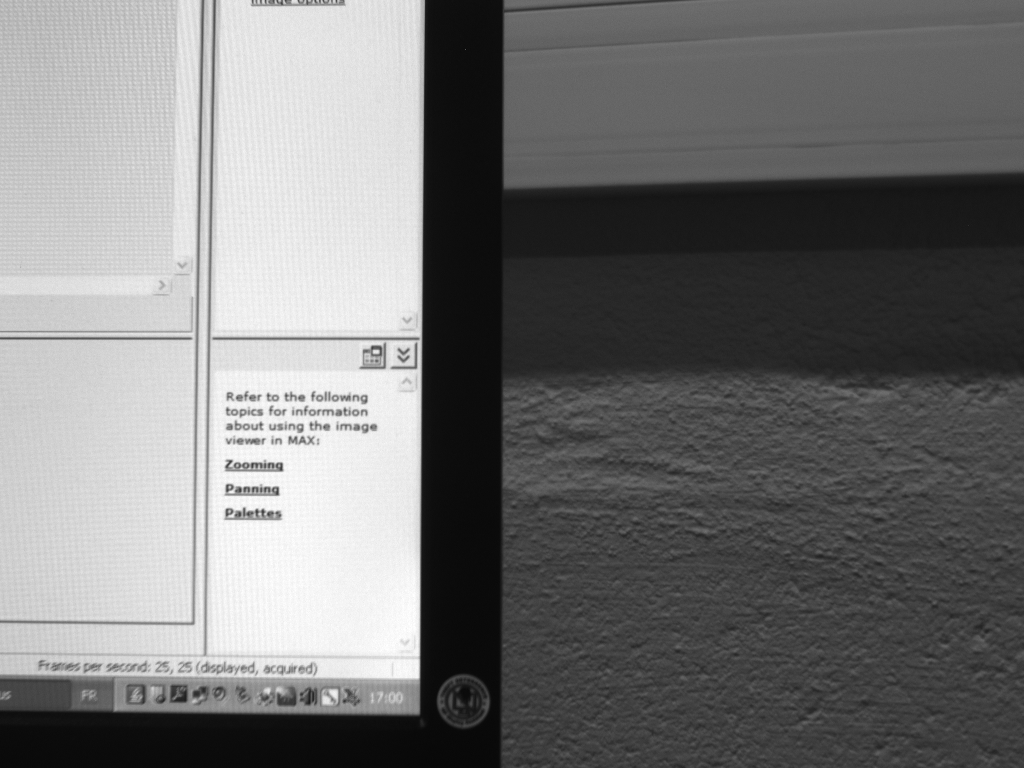
\includegraphics[width=1.0\textwidth,natwidth=100,natheight=100]{../CPM/im0-1pol.png}
  \caption{Image after 1st polarizer}
  \label{fig:cpm1-1}
\end{minipage}
\quad
\begin{minipage}[b]{0.3\linewidth}
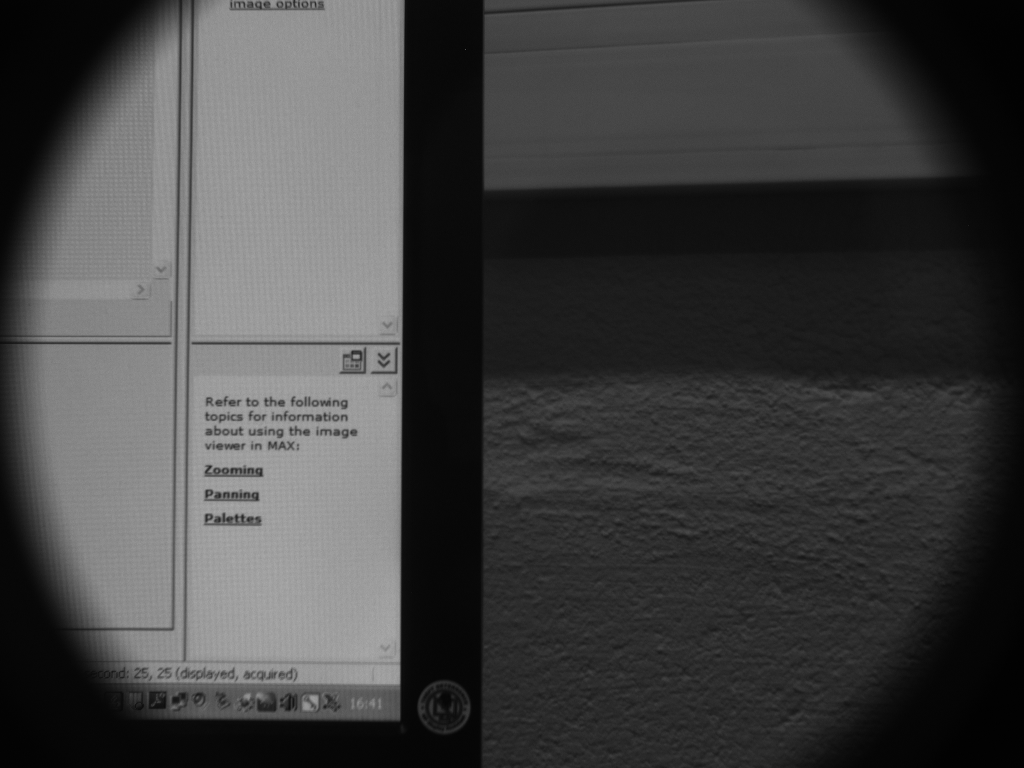
\includegraphics[width=1.0\textwidth,natwidth=100,natheight=100]{../CPM/im0.png}
  \caption{Image after both polarizers at 0}
  \label{fig:cpm1-2}
\end{minipage}
\quad
\begin{minipage}[b]{0.3\linewidth}

\includegraphics[width=1.0\textwidth,natwidth=100,natheight=100]{../CPM/im90.png}
  \caption{Image after both polarizers at 90}
  \label{fig:cpm1-3}
\end{minipage}
\end{figure}

The next step was to introduce the TNLC rotator to see its effect. 
We know that this device should act as a "switch" for the polarization
rotation: one state when no voltage is applied and the other when the maximum
voltage is applied. However, we didn't know the angle of rotation in either
of the states. 

For this, we placed the TNLC in the middle and take 2 measurements: first
with 0v and another with a maximum voltage (see figures \ref{fig:cpm2-1} and
\ref{fig:cpm2-2}).

We observed
that when no voltage was applied, we got a black image. We could infere then that
at 0V the TNLC was orthogonally oriented with respect of the polarizers, which means
it was oriented at 90$^\circ$. Similarly, when we applied the maximum
voltage, we got the maximum intensity and therefore we can deduce it was aligned
with the other two polarizers at 0$^\circ$.

\begin{figure}[H]
\centering
\begin{minipage}[b]{0.45\linewidth}
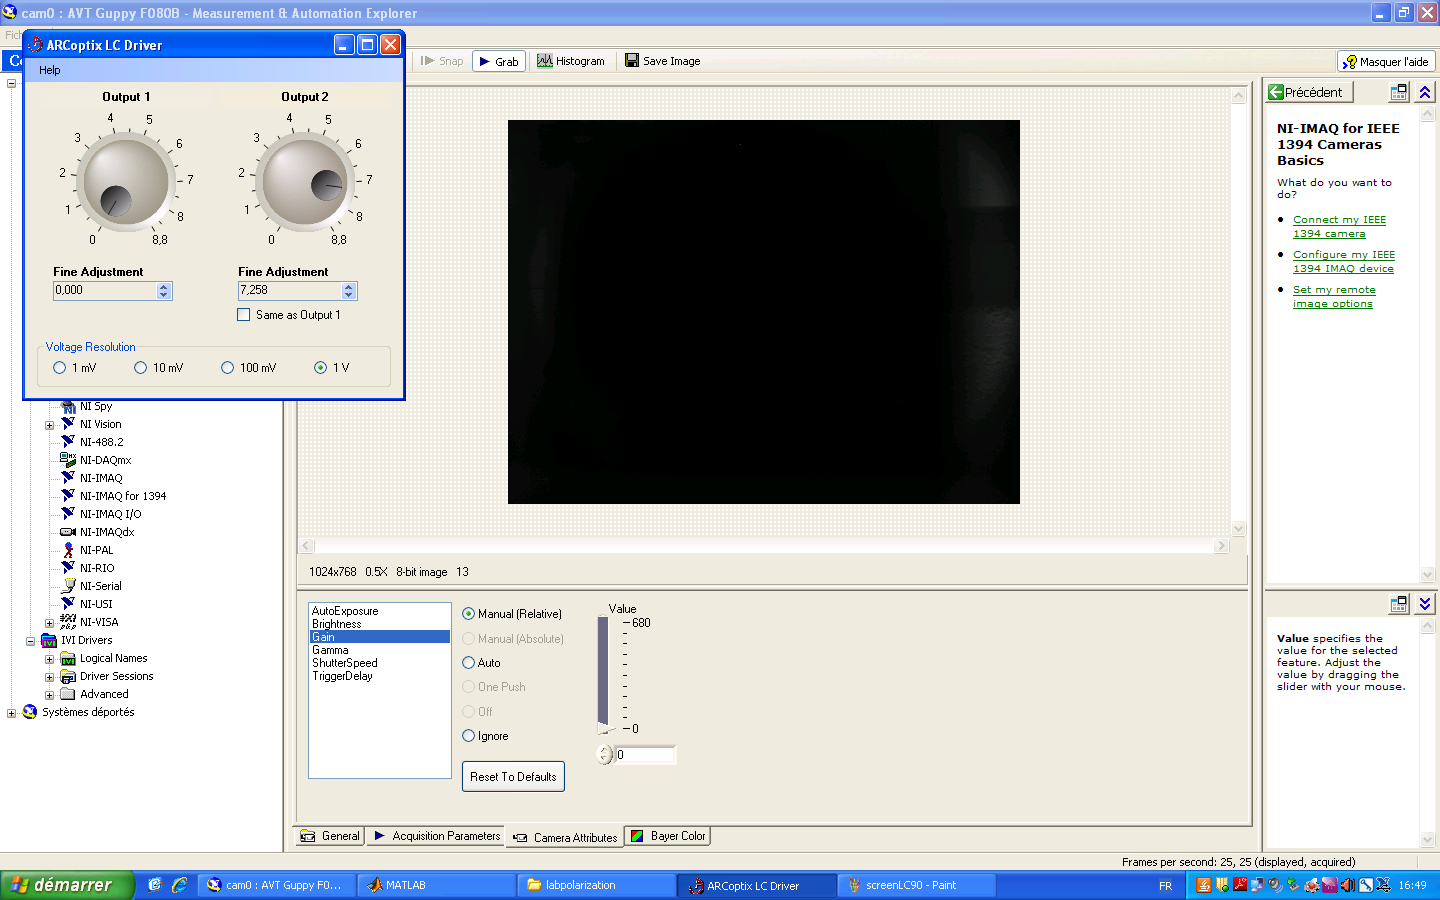
\includegraphics[width=1.0\textwidth,natwidth=100,natheight=100]{../CPM/screenLC0.PNG}
  \caption{TNLC at 0V }
  \label{fig:cpm2-1}
\end{minipage}
\quad
\begin{minipage}[b]{0.45\linewidth}
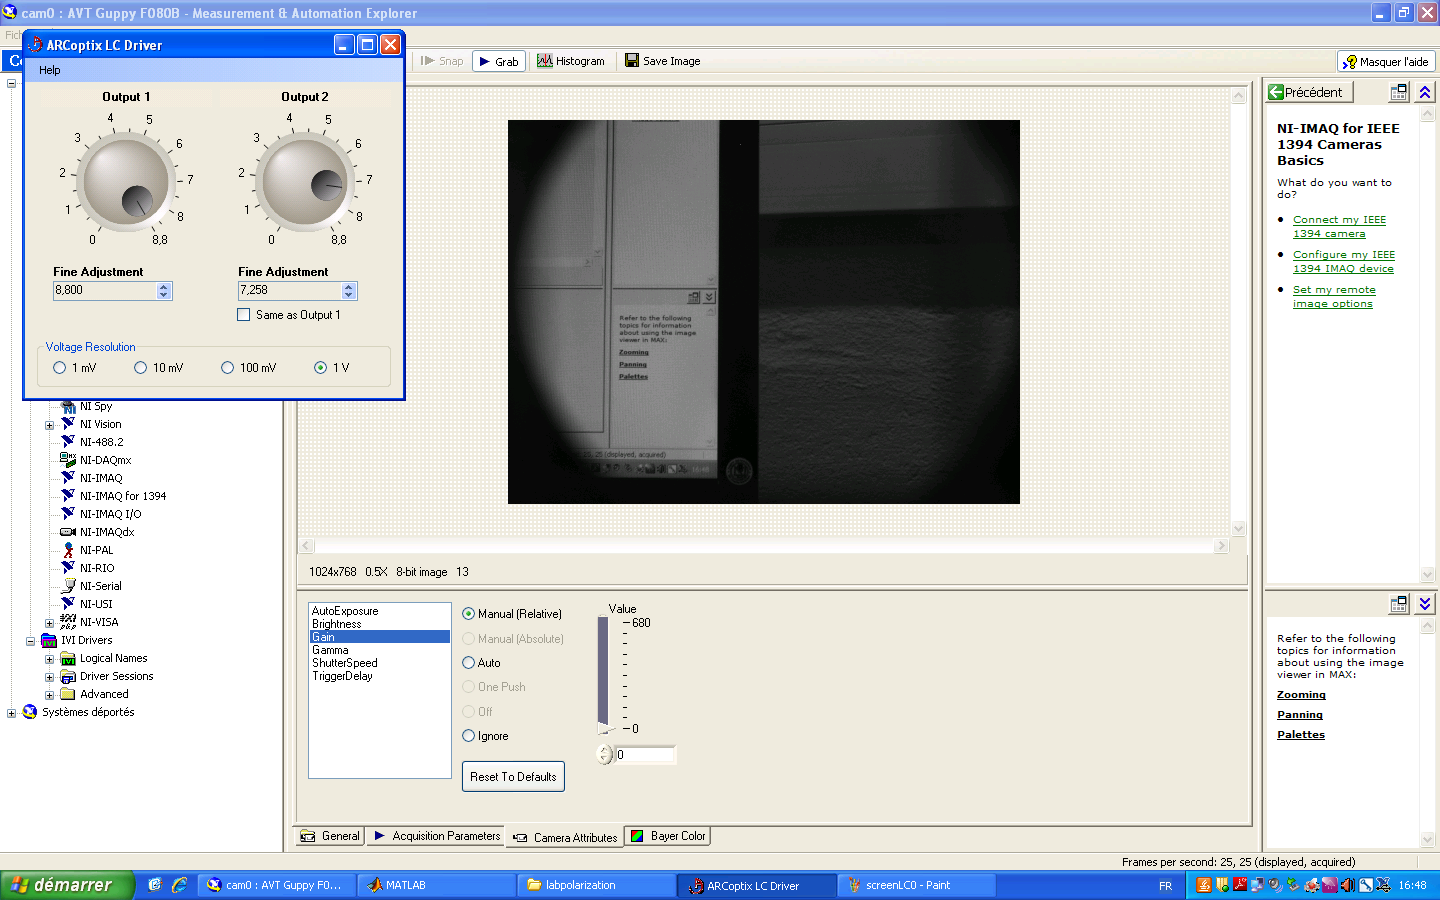
\includegraphics[width=1.0\textwidth,natwidth=100,natheight=100]{../CPM/screenLC90.PNG}
  \caption{TNLC at Max V}
  \label{fig:cpm2-2}
\end{minipage}
\end{figure}

\section{Difuse Specular Reflection}

The idea of this section was to make use of the effect of specular and difuse reflection
over linearly polarized light.
We knew that difuse reflection causes that the incident linearly polarized light 
becomes unpolarized and that specular reflection preserves the polarization. 
That is why, in order to get rid of the specular reflection, we only needed to 
cancel it out by rotating the polarized light 90$^\circ$ with respect to
the polarizer. This was achieved by using the TNLC.

First, we aligned the polarizer used in front of the light with the polarizer in front
of the camera. This means that the generated linearly polarized light was paralel to the 
polarizer . 

The first picture was taken by applying the maximum voltage to the
TNLC so that no rotation was performed on the incident linearly polarized light. This meant that 
both, incident polarized light and polarizer were parallel (figure \ref{fig:cpm3-1} left).

For the second picture, no voltage was applied on the TNLC, and therefore a 90$^\circ$
was performed on the linearly polarized light (figure \ref{fig:cpm3-1} right), therefore
the specular reflection was cancelled.


\begin{figure}[H]
\centering
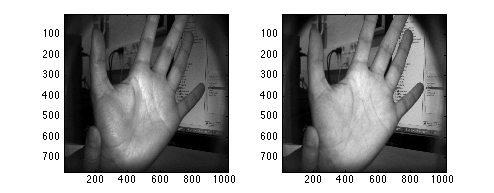
\includegraphics[width=0.7\textwidth,natwidth=100,natheight=100]{../CPM/Difuse/difnodif.png}
  \caption{Image 1 Rotator at }
  \label{fig:cpm3-1}
\end{figure}
The calculated parameters for total light intensity, polarization contrast and polarization
contrast ratio are shown in the figure \ref{fig:cpm3-2}. All the images were shown by
scaling the obtained intensity except for the bottom right one. We wanted to enhance the 
polarized areas in the polarization contrast image by just discarding the negative values and 
then negating the image. Here we could clearly visualize that the black 
portion of the picture corresponds 
to the specular reflection.
\begin{figure}[H]
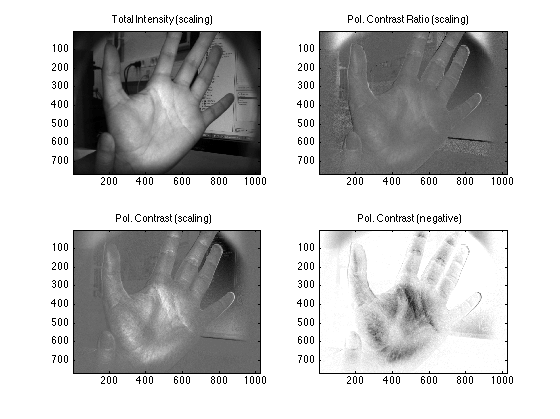
\includegraphics[width=1.0\textwidth,natwidth=100,natheight=100]{../CPM/Difuse/difparams.png}
  \caption{Image 1 filtered (without specular reflection)}
  \label{fig:cpm3-2}
\end{figure}

\bibliographystyle{plain}
\bibliography{biblio}
\end{document}
